% ============================ Enrico Ribiani 16-03-2021 ====================================================================
% Base per i documenti  
\documentclass[12pt]{article}
% ------------ pacchetti necessari ----------------
\usepackage[a4paper, total={6in, 8in},margin=1in]{geometry} % formattazione decente della pagina
\usepackage{graphicx}                            % need for figure
\usepackage{amsmath}
\usepackage{amsfonts}                            % if you want the fonts
\usepackage{amssymb}                             % if you want extra symbols
\usepackage{graphicx}  
\renewcommand{\figurename}{Figura}                          % need for figures
\usepackage{mathptmx}
\usepackage{float}                               % serve per mettere tabelle e immagini dove si vuole 
\usepackage[utf8]{inputenc}
\usepackage{textcomp}
\usepackage[hang,flushmargin,bottom]{footmisc}   % footnote format
\usepackage{fancyhdr, lastpage}
\usepackage{titlesec}

\usepackage[table,dvipsnames]{xcolor}
\pagestyle{fancy}
\renewcommand{\headrulewidth}{0pt}
\renewcommand*\contentsname{Indice}
\titleformat{\section}{\normalsize\bfseries}{\thesection.}{1em}{}	% required for heading numbering style
\titleformat*{\section}{\Large\bfseries}
\titleformat*{\subsection}{\large\bfseries}
\usepackage{tikz}
\usetikzlibrary{arrows,shapes,positioning,shadows,trees}

%===================links=================
\usepackage{hyperref}
\hypersetup{
    colorlinks=true,
    linkcolor=Sepia,
    filecolor=Green,      
    urlcolor=Cyan,
    pdftitle={SAMPLE},
    pdfpagemode=FullScreen,
    }
    \usepackage{pdfpages}
    \usepackage{float}
    \usepackage{placeins}
    \usepackage{mwe} % for blindtext and example-image-a in example
    \usepackage{wrapfig}
    %===================inizio pagina del titolo=================
\begin{document}
    \begin{titlepage}
\begin{flushleft}
\vspace{3\baselineskip}

\Huge{\textbf{Impianto domotico con punto luce e tapparella gestito da telecomando.}}
\vfill
\LARGE Enrico Ribiani\\
\LARGE 4AUB\\
\vfill
\huge{ITT M. BUONARROTI 09-11-2021}

%=============== fine pagina titolo ===============
\end{flushleft}
\end{titlepage}
%=============== Intestazione ===============
\pagestyle{fancy}
\fancyhead{}
\fancyhead[RO,LE]{Enrico Ribiani}
\fancyhead[LO,RE]{4AUB}

%\fancyhead[CO,CE]{sezione \thesection}%??????????????''
%=============== fine Intestazione ===============

\tableofcontents
\vskip 3cm
\section{Introduzione}
Nelle ore di laboratorio di Sabato 30 ottobre abbiamo montato questo impianto domotico utilizzando i componenti Tixya di DeltaDore 
con l'obiettivo di comandare tramite un telecomando una tapparella e un punto luce accendibile anche da un pulsante.

%\section{Guida all'uso}
\section{Lista materiale/Preventivo}
Per comandare la tapparella abbiamo usato il modulo che funge da attuatore \textit{Tyxia 5730},
mentre per il punto luce abbiamo utilizzato il modulo \textit{Tyxia 5610}, mentre per comunicare con entrambi abbiamo utilizzato
il telecomando \textit{Tyxia 1712} che permette di essere associato ad entrambi i moduli e comandare tapparelle e punto luce 
con lo stesso telecomando cambiando modalità.\\
Per simulare una taparella sono state usate due spie led, una per simulare la tapparella che salire e una per simulare la tapparella scendere, per 
il punto luce è stata utilizzata una lampadina comandata anche da un pulsante, il tutto è stato collegato con fili di rame da 1,5 mm.
\vfill    
\subsection{Tabella preventivo}
    \begin{table}[H]
        \begin{tabular}{||c|c|c|c|c|c|}
            \hline
            \rowcolor{RawSienna!80} Codice prodotto & Dispositivo & Descrizione & Quantità & Prezzo & Totale \\
            \hline
            \rowcolor{Orange!70} Tyxia 5730 & Ricevitore & Attuatore luci & 1 & 80 & 80 \\
            \hline
            \rowcolor{TealBlue!70} Tyxia 5610 & Ricevitore & Attuatore tapparelle & 1 & 60 & 60 \\
            \hline
            \rowcolor{Orange!70} Tyxia 1712 & telecomando & Telecomando a canale multiplo & 1 & 130 & 130 \\
            \hline
            \rowcolor{TealBlue!70}  & pulsante & controllo non wireless luce & 1 & 5 & 5 \\
            \hline
            \rowcolor{Orange!70}  & lampadina & punto luce & 1 & 4 & 4 \\
            \hline
        \end{tabular}
        \vspace{1cm}
        \begin{center}
            
        \begin{tabular}{|p{2cm}|}
            
            \hline
            \rowcolor{RawSienna!80} Totale\\
            \hline
            \rowcolor{Orange!70} 269\\
            \hline            
        \end{tabular}
    \end{center}

    \end{table}
    \FloatBarrier
\section{Montaggio}
Prima di iniziare a montare dobbiamo assicurarci di avere a portata di mano tutti i datasheet dei componenti 
utilizzati, per avere un'ulteriore sicurezza nella conoscenza del componente sebbene si riesca a capire cosa vada
collegato ai morsetti senza perchè sono tutti chiaramente segnati.\\
I datasheet sono particolarmente utili nella parte di associazione che andremo a trattare in seguito.\\
Per il montaggio abbiamo utilizzato i colori normalizzati secondo la CEI 16-4, quindi marrone per la fase, blu chiaro
per il neutro, giallo verde per la terra e rosso per uso generale.\\
\begin{wrapfigure}{l}{0.5\textwidth}
    \centering
    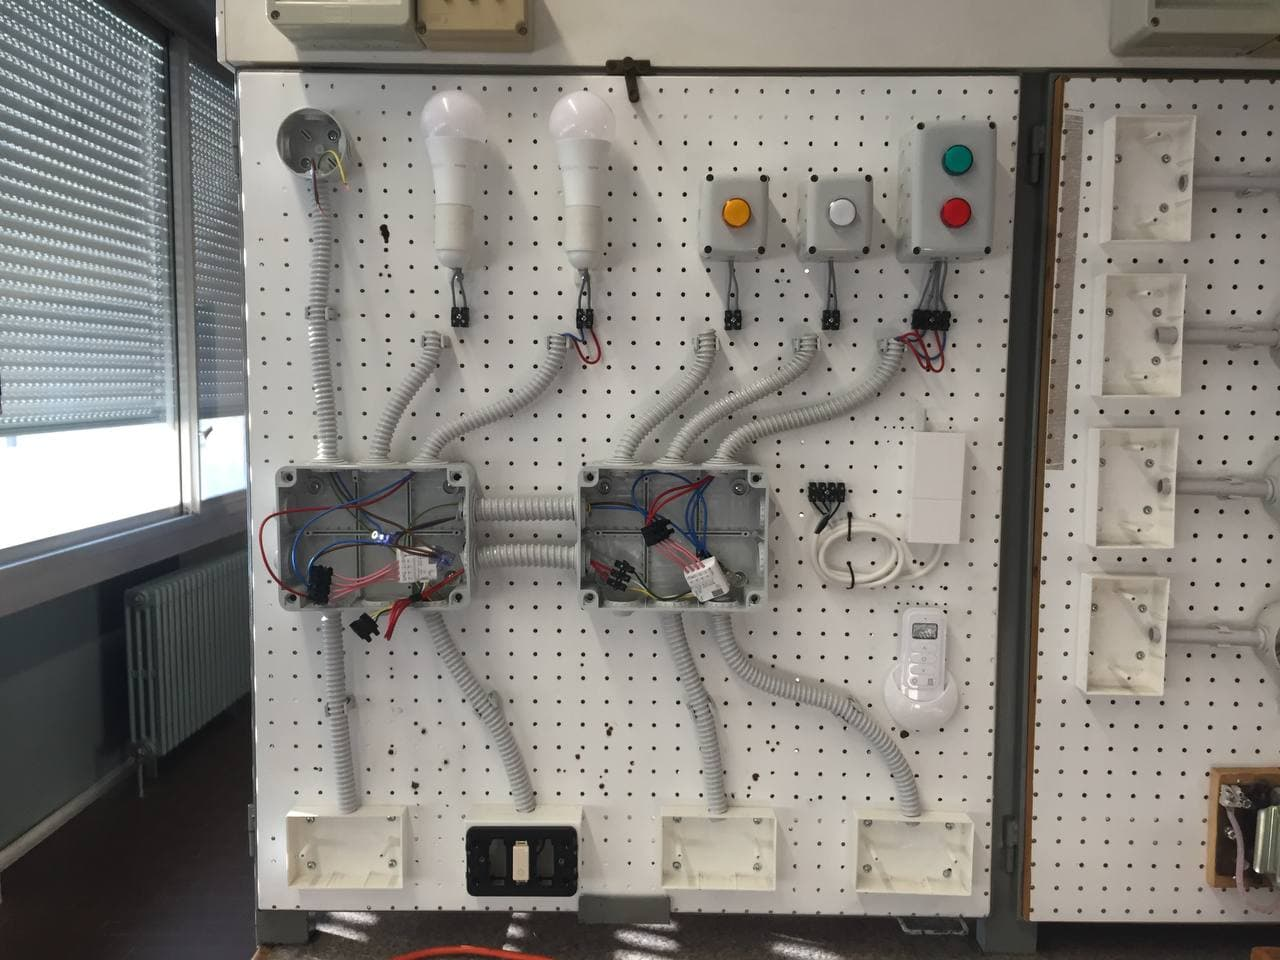
\includegraphics[width=.98\linewidth]{/home/rib/Documenti/latec/TPSE-domotica-14-11-2021/media/foto-montaggio.jpg}
    \end{wrapfigure}
Ho iniziato a cablare prima le parti con dei morsetti fissati come le spie delle tapparelle e la lampadina, dopodichè 
ho collegato questi componenti ai rispettivi moduli, ossi a il 5730 per le tapparelle e il 5610 per il punto luce.\\
Successivamente ho collegato il pulsante al 5610 e ho proceduto a collegare fase e neutro per entrambi i moduli facendo un ponte
sia sulla fase che sul neutro per collegarli entrambi.\\
Anche se non è stata utilizzato ho tirato la terra fino alla scatola di derivazione\\
Una volta verificato i collegamenti ho acceso l'impianto e prima di collaudarlo ho effettuato l'associazione.\\
    
    
    
    \clearpage

    \subsection{Associazione}
    Per questa esperienza la parte di associazione non è stata subito intuitiva perché i moduli andavano associati al 
    telecomando uno allla volta ricordandosi di dare conferma alla fine, bisogna ricordarsi di consultare in modo 
    opportuno i datasheet per capire come e quale modalità di associazione funge meglio per le proprie necessità.\\
\section{Datasheets}
\begin{itemize}
    \item \href{https://www.deltadore.fr/data/product_files/6351400/documents/notices/Install/fr/web_2704527_rev5_not_nano_TYXIA_5610_5612_FR-rev05.pdf}{tyxia 5610}
    \item \href{https://www.deltadore.fr/data/product_files/6351402/documents/notices/Install/fr/web_2704526_rev5_not_nano_TYXIA_5630_5730_FR-rev05.pdf}{tyxia 5730}
    \item \href{https://www.deltadore.fr/data/product_files/6351406/documents/notices/Install/fr/web_2704633_rev3_Telecommande_TYXIA_1712_FR-rev03.pdf}{tyxia 1712}
\end{itemize}
    \section{Allegati}
    \subsection{Schema di montaggio}
    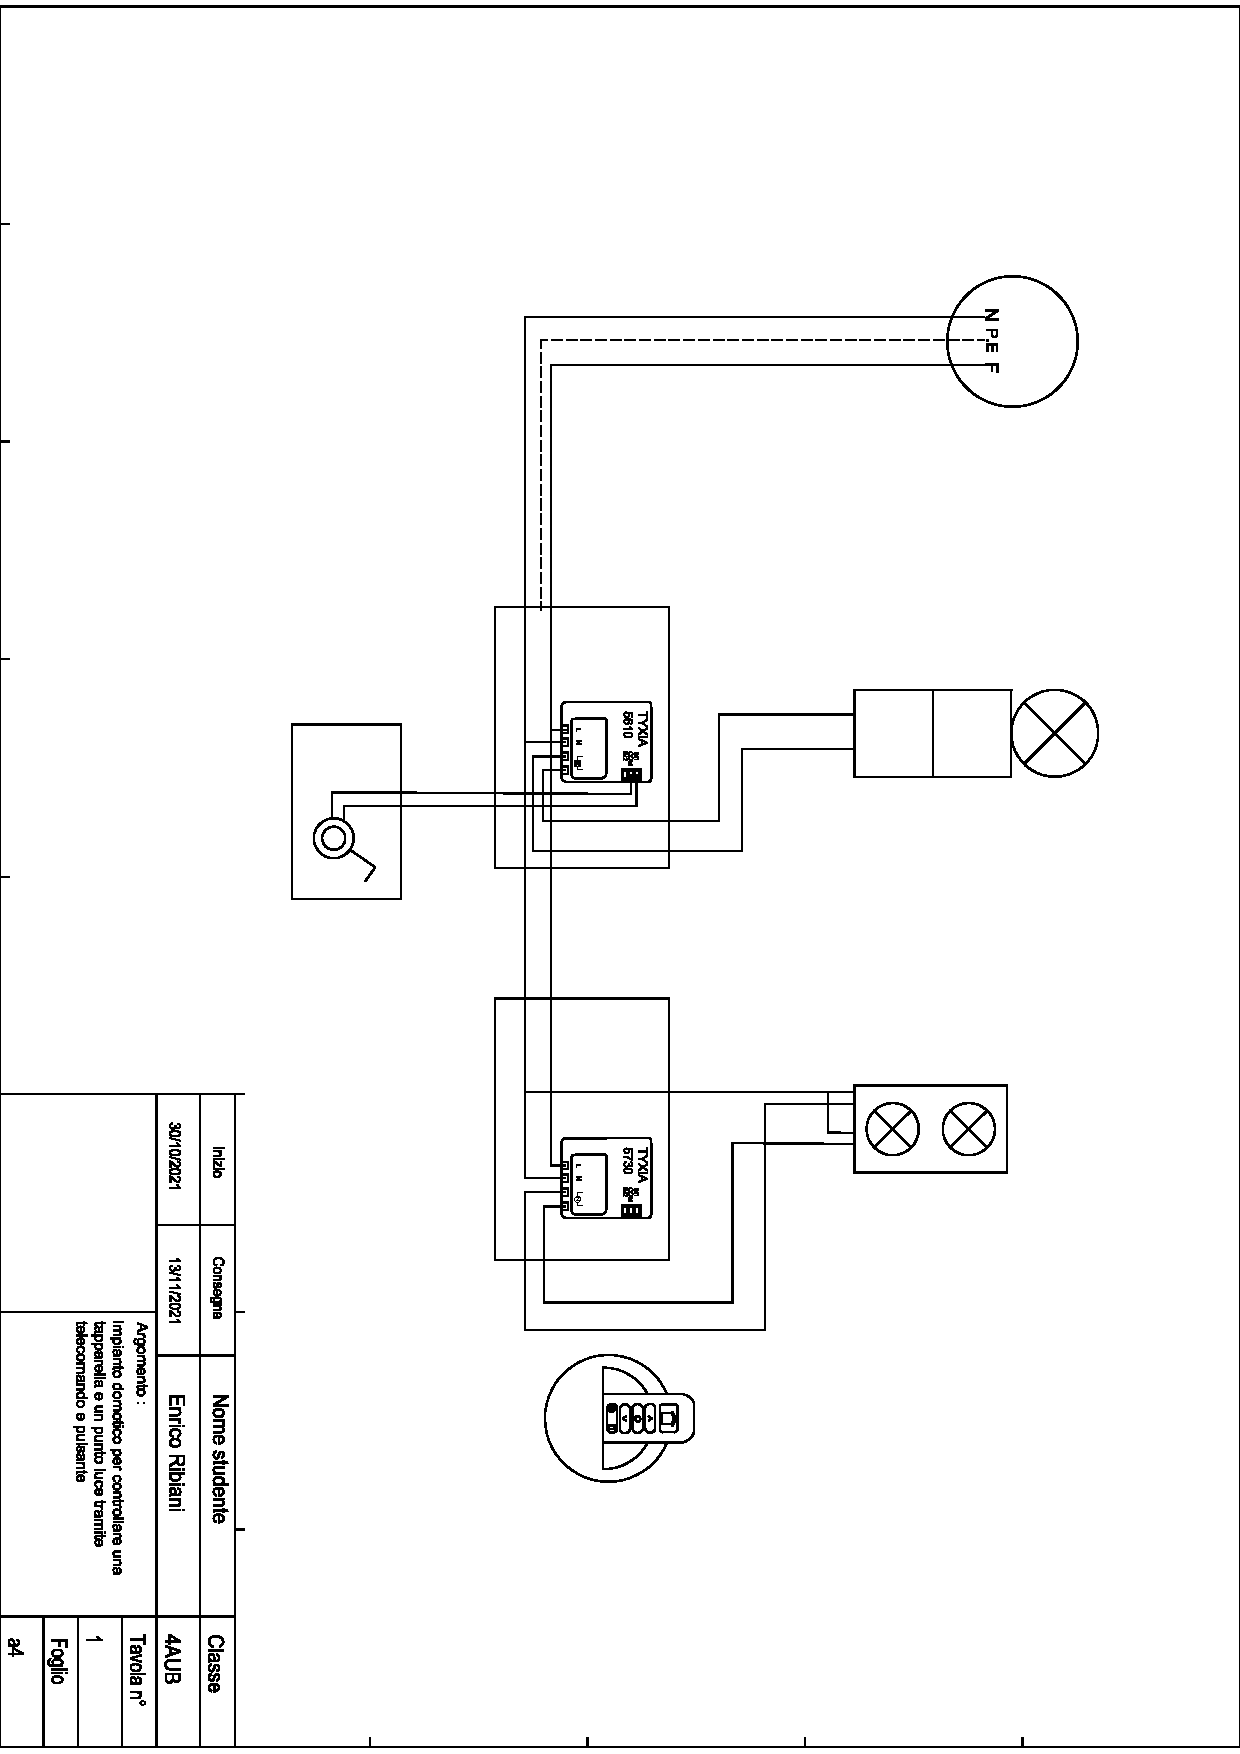
\includepdf[pages={1}]{/home/rib/Documenti/latec/TPSE-domotica-14-11-2021/media/tavla.pdf}
\end{document}